% *neode.onsave* setgo rm draft.pdf; xelatex -interaction=nonstopmode draft; biber draft; xelatex -interaction=nonstopmode draft; xelatex -interaction=nonstopmode draft; evince draft.pdf

\documentclass[bachelor]{kththesis}

\usepackage{csquotes} % Recommended by biblatex
\usepackage{biblatex}
\addbibresource{sources.bib} % The file containing our references, in BibTeX format

\usepackage{chngcntr}
\counterwithout{figure}{chapter}
\counterwithout{figure}{section}

\usepackage{color}
\usepackage{graphicx}
\usepackage{float}
\usepackage{algorithm2e}

\newcommand{\blue}[1]{{\color{blue} [#1]}}
\newcommand{\red}[1]{{\color{red} [#1]}}

\title{A performance survey of coverage algorithms for simple robotic vacuum cleaners}
\alttitle{En prestandaundersökning av täckningsalgoritmer för enkla robotdammsugare}
\author{Robin Gunning}
\email{rgunning@kth.se}
\supervisor{Jana Tumova}
\examiner{Örjan Ekeberg}
\programme{Bachelor's degree in Computer Science}
\school{School of Computer Science}
\date{\today}


\begin{document}

% Frontmatter includes the titlepage, abstracts and table-of-contents
\frontmatter

\titlepage

\begin{abstract}
  English abstract goes here.
\end{abstract}


\begin{otherlanguage}{swedish}
  \begin{abstract}
    Abstrakt på svenska.
  \end{abstract}
\end{otherlanguage}


\tableofcontents


% Mainmatter is where the actual contents of the thesis goes
\mainmatter


\chapter{Introduction}
% We use the \emph{biblatex} package to handle our references.  We therefore use the
% command \texttt{parencite} to get a reference in parenthesis, like this
% \parencite{heisenberg2015}.  It is also possible to include the author
% as part of the sentence using \texttt{textcite}, like talking about
% the work of \textcite{einstein2016}.

Most cheap automatic robot vacuum cleaners (from here on called robot cleaner) today combines three 
or four different path planning algorithms to get the expected coverage as fast as possible. This 
has sparked the interest to develop efficient algorithms to reduce cleaning time and be as efficient 
as possible.
  
There are several types of robot cleaners of available to the public today, however the price range 
of these robot cleaners varies greatly and there is no set standard of what sensors a robot cleaner 
should have. This makes almost every robot cleaner unique in the way of getting a good coverage of 
the room it is supposed to clean. Furthermore different robot cleaners and companies has their own 
algorithms developed to maximize coverage and minimizing the dust on the floor. 
\\\\
Usually the price of the robot cleaner seems to correlate with the number of sensors and how 
advanced the sensors are \parencite{irobot}. Cheaper models often only have a single sensor which 
is a frontal bumper (Figure.~\ref{fig:skantic}), a micro switch which gets pressed when the robot cleaner bumps in to a 
wall or another object. 

\begin{figure}[H]
	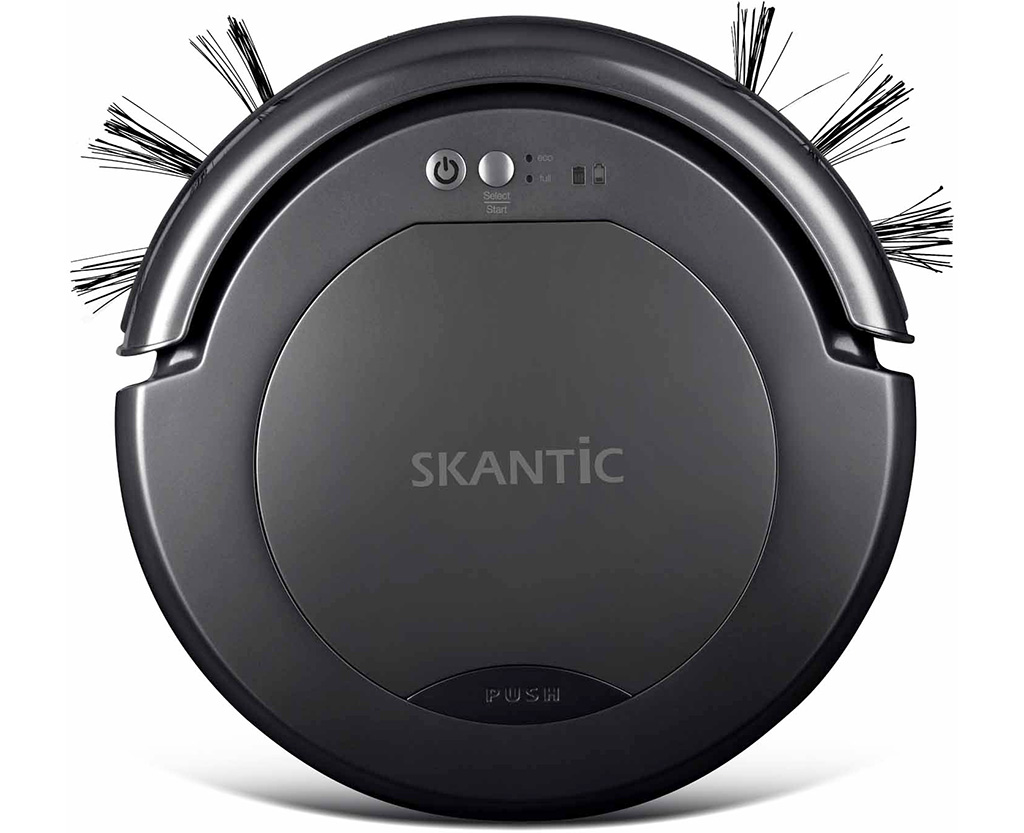
\includegraphics[width=3cm]{img/cheap.jpg}
	\centering
	\label{fig:skantic}
	\caption{Skantic Robot Cleaner 10 \parencite{scantic}}
\end{figure}

\noindent More expensive models often utilize optical sensors to measure how many times the 
wheels have rotated and some models even use lasers and radar to build virtual maps of the rooms the 
robot cleaner operate in.
Rooms come in all different sizes and shapes and different algorithms are likely to have different 
strengths depending on the type of room. The standard algorithms for cheap robot cleaners are 
Boustrophedon, random walk, spiral and wall follow \parencite{hasan}.

Boustrophedon travels forward until hitting a wall, when hitting the wall the robot reverses for a 
while then turns 90 degrees clockwise or counter clockwise then travels for a short period and turns
another 90 degrees in the same direction as chosen when hitting the wall.
That makes the robot cleaner do an 180 degrees turn while not cleaning the same space twice. 
When reaching the opposite wall the robot cleaner performs the same set of instructions as before 
but in the opposite direction. This makes the robot cleaner zig-zag between two walls while traversing the room.

Random walk turns a random amount of degrees and travels in a straight path until it hits a wall. 

Spiral is a counter clockwise spiral from in to out and wall follow when hitting a wall travels in 
a small half circle until it hit the wall again and continues doing this around the room or until 
the robot cleaner switches algorithm \parencite{hasan}. 




\chapter{Background}

\section{Previous research}


Most previous research seem to use cellular decomposition which divides the 
room into several cells and performs the algorithm in each cell. Each cell is made up of a part of the room, making a new cell at the critical point for each room. The critical point is where the connectivity of a cell changes, for example when an obstacle divides the room. According to \textcite{choset},
fewer cells are better as fewer number of cells minimize the number of zig-zag motions the robot has to make, but more cells are guaranteeing the robot exhaustively covers the entire environment however this can be countered by making the boustrophedon algorithm have a shorter ''side step''.

Some previous research has been done in the field of comparing different algorithms for unexplored 
environments and while the best coverage per minute is achieved when using all the algorithms 
combined, boustrophedon is the next best performing algorithm \parencite{
}. 

Boustrophedon cellular decomposition is where the environment is decomposed into smaller cells which makes it easier to get more coverage.
Combining cellular decomposition with graph theory to generate an Euler tour
guarantees complete coverage of the known work space while minimizing the traveled path by 
the robot. \parencite{rekl}.
Using landmark-based topological coverage or grid-based methods improves the coverage of algorithms like boustrophedon  \parencite{galceran}.


\subsection{Algorithms}

This section contains background of the studies and used algorithms for this thesis.

\subsubsection{Boustrophedon}
Boustrophedon means ox-turning in ancient Greek, and mimics an ox when plowing and makes the robot zig-zag from opposite walls while traversing the room length wise\parencite{choset}\parencite{rekl}. The pseudocode (Algorithm.~\ref{alg:bous}) is a direct translation from the boustrophedon flowchart from \textcite{hasan}. The algorithm starts by going upwards and then makes the robot cleaner turn 90 degrees right 
when the front bumper is triggered, and then travels a distance equal to the robot cleaners diameter 
and turns 90 degrees right again making the robot face downwards. The robot cleaner then travels downwards till the bumper is 
triggered again. The robot cleaner will now turn 90 degrees left,
and then travels a distance equal to the robot cleaners length and turns 90 degrees left again making the robot cleaner face upwards. After this the algorithm restarts. The path generated by the algorithm is depicted by (Figure.~\ref{fig:2}).
\\\\
\begin{algorithm}[H]
	\SetAlgoLined
	Start direction up
	
	Let one roboUnit = the diameter of the robot
	
	\eIf{collision detected}{
		
		Move backwards one roboUnit
		
		\eIf{if count is odd}{
			Turn 90 degrees clockwise
			
			Move forwards one roboUnit
			
			Turn 90 degrees clockwise
			
			add 1 to count
		}
		{
			Turn 90 degrees counter clockwise
			
			Move forwards one roboUnit
			
			Turn 90 degrees clockwise
			
			add 1 to count
		}
	}
	{
		Move forwards
	}	
	\caption{Boustrophedon \parencite{hasan}}
	\label{alg:bous}

\end{algorithm}


\begin{figure}[H]
	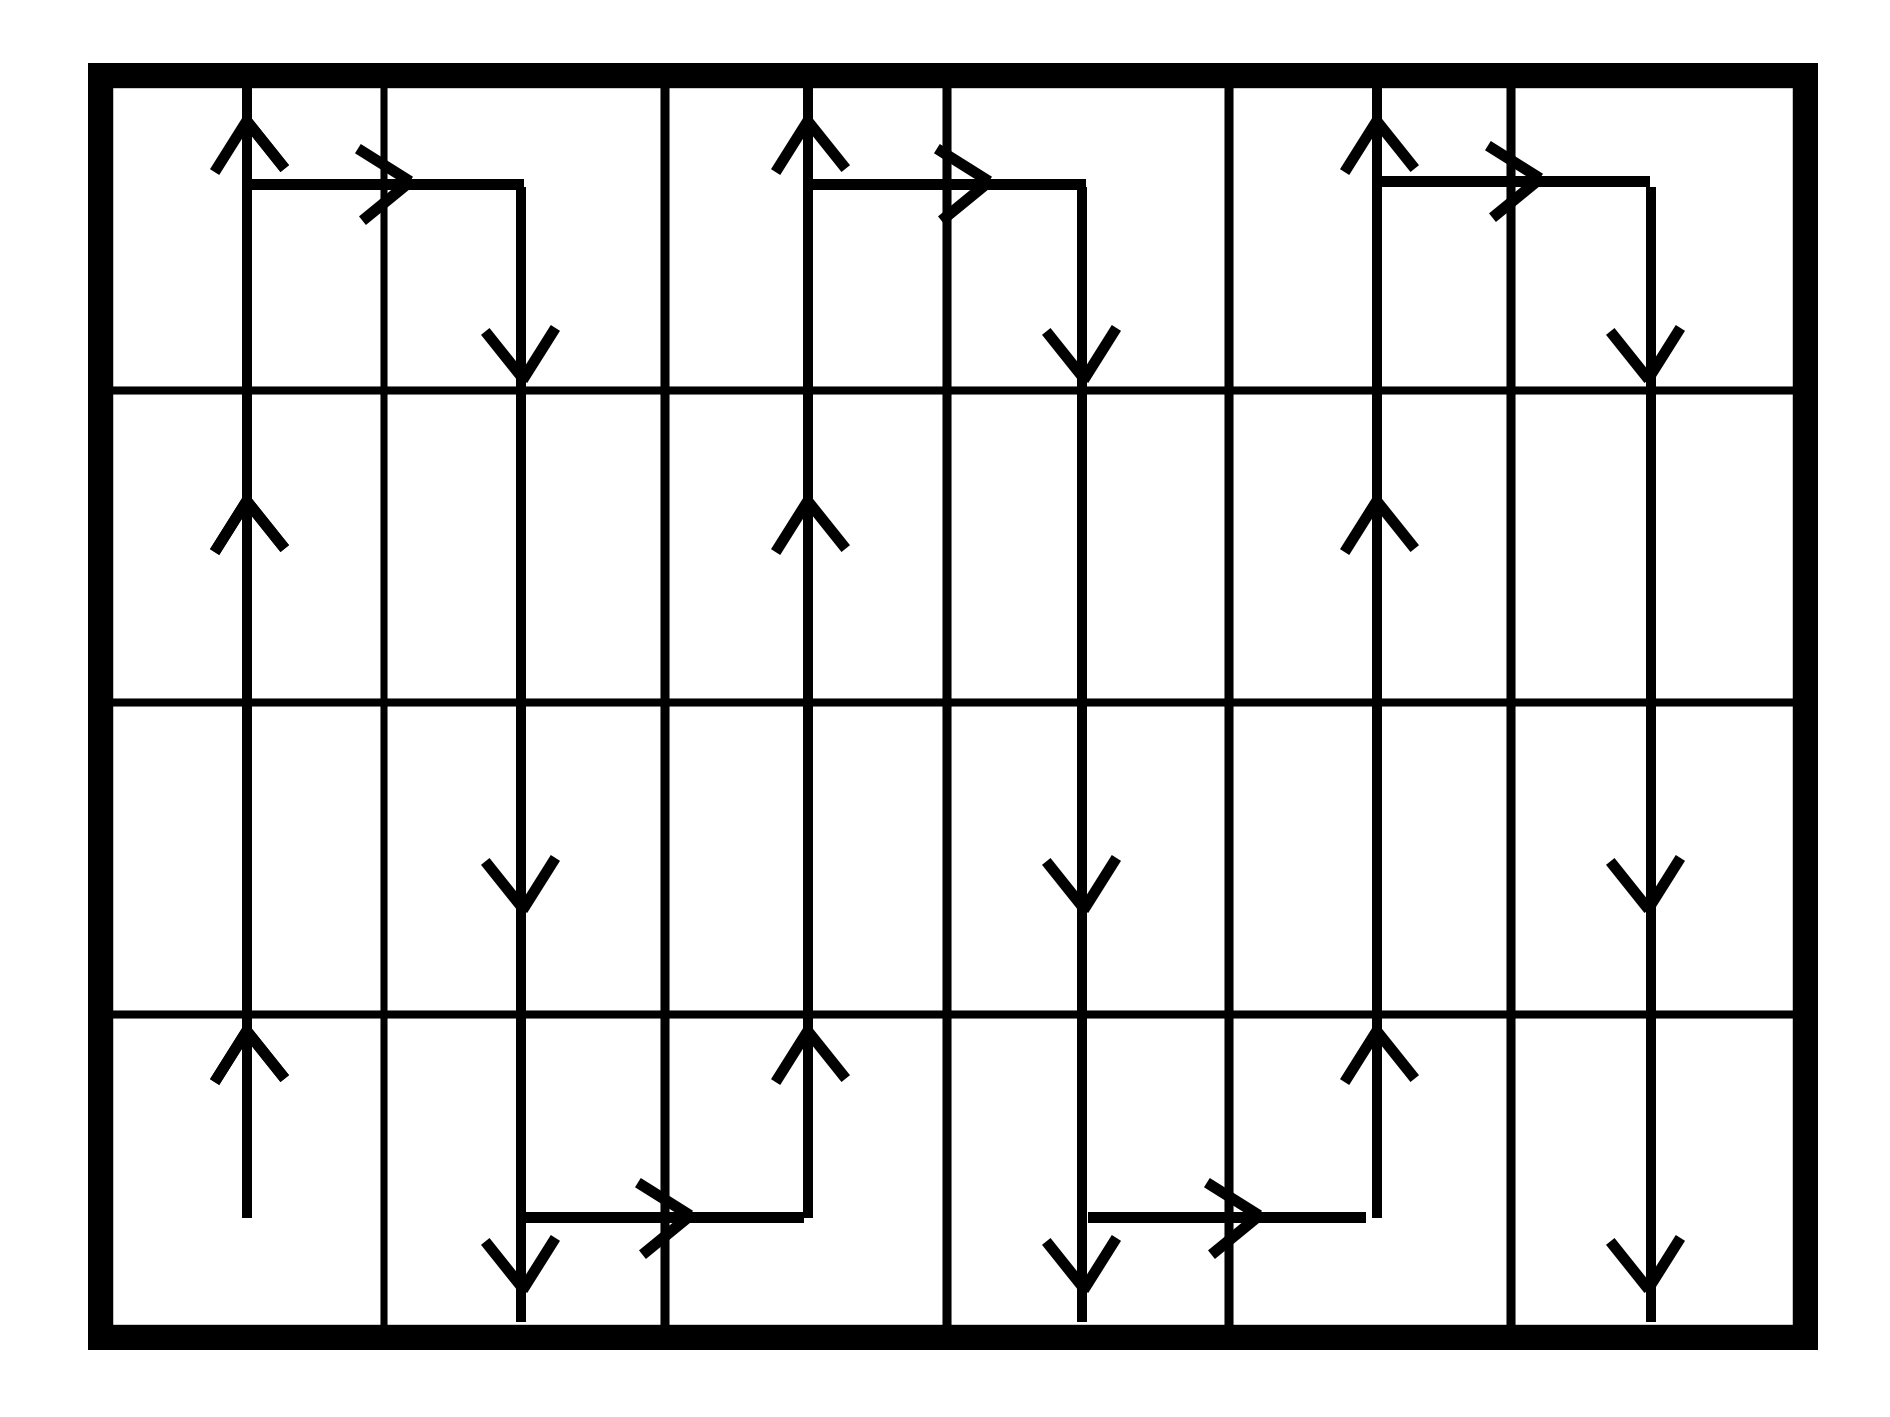
\includegraphics[width=5cm]{img/bous.png}
	\centering
	\caption{Boustrophedon}
	\label{fig:2}
\end{figure}


\noindent In the case where the room/space is known beforehand the boustrophedon algorithm gains a lot from dividing the room into smaller parts for better coverage. As the obstacles and furnitures in the room are known and divided into cells where the obstacles are, the robot cleaner can easily plan it's boustrophedon path for every cell. When all the cells have been visited and cleaned, the entire room is cleaned \parencite{choset}. There is a difference between following the longer or the shorter wall of the room, there will be no difference in coverage however there are some small gains if the robot cleaner follows the long wall of the room as the robot cleaner does not have to make as many turns as when following the short wall which saves battery.
\\\\

\subsubsection{Spiral}
The spiral algorithm makes the robot cleaner move in an increasing spiral path. This algorithm works best if the robot is placed in the middle of the room and has enough space to perform the spiral correctly. When the robot cleaner starts this algorithm it starts a right or left hand side spiral from the center point outwards until it the front bumper is triggered. 
 The pseudocode (Algorithm.~\ref{alg:spiral}) is a direct translation from the spiral flowchart from hasan's report \parencite{hasan}.
\\\\
\begin{algorithm}[H]
	\SetAlgoLined
	\While{no collision}{
		Move forward
		
		Turn right according to turning angle
		
		Decrease turning angle
	}

	\caption{Spiral \parencite{hasan}}
	\label{alg:spiral}
	
\end{algorithm}
\bigskip
When that happens the robot cleaner stops the spiral algorithm and proceeds with another algorithm since starting the spiral algorithm when close to a wall is meaningless \parencite{hasan}.
The path generated by the algorithm is depicted by (Figure.~\ref{fig:3}).
\begin{figure}[H]
	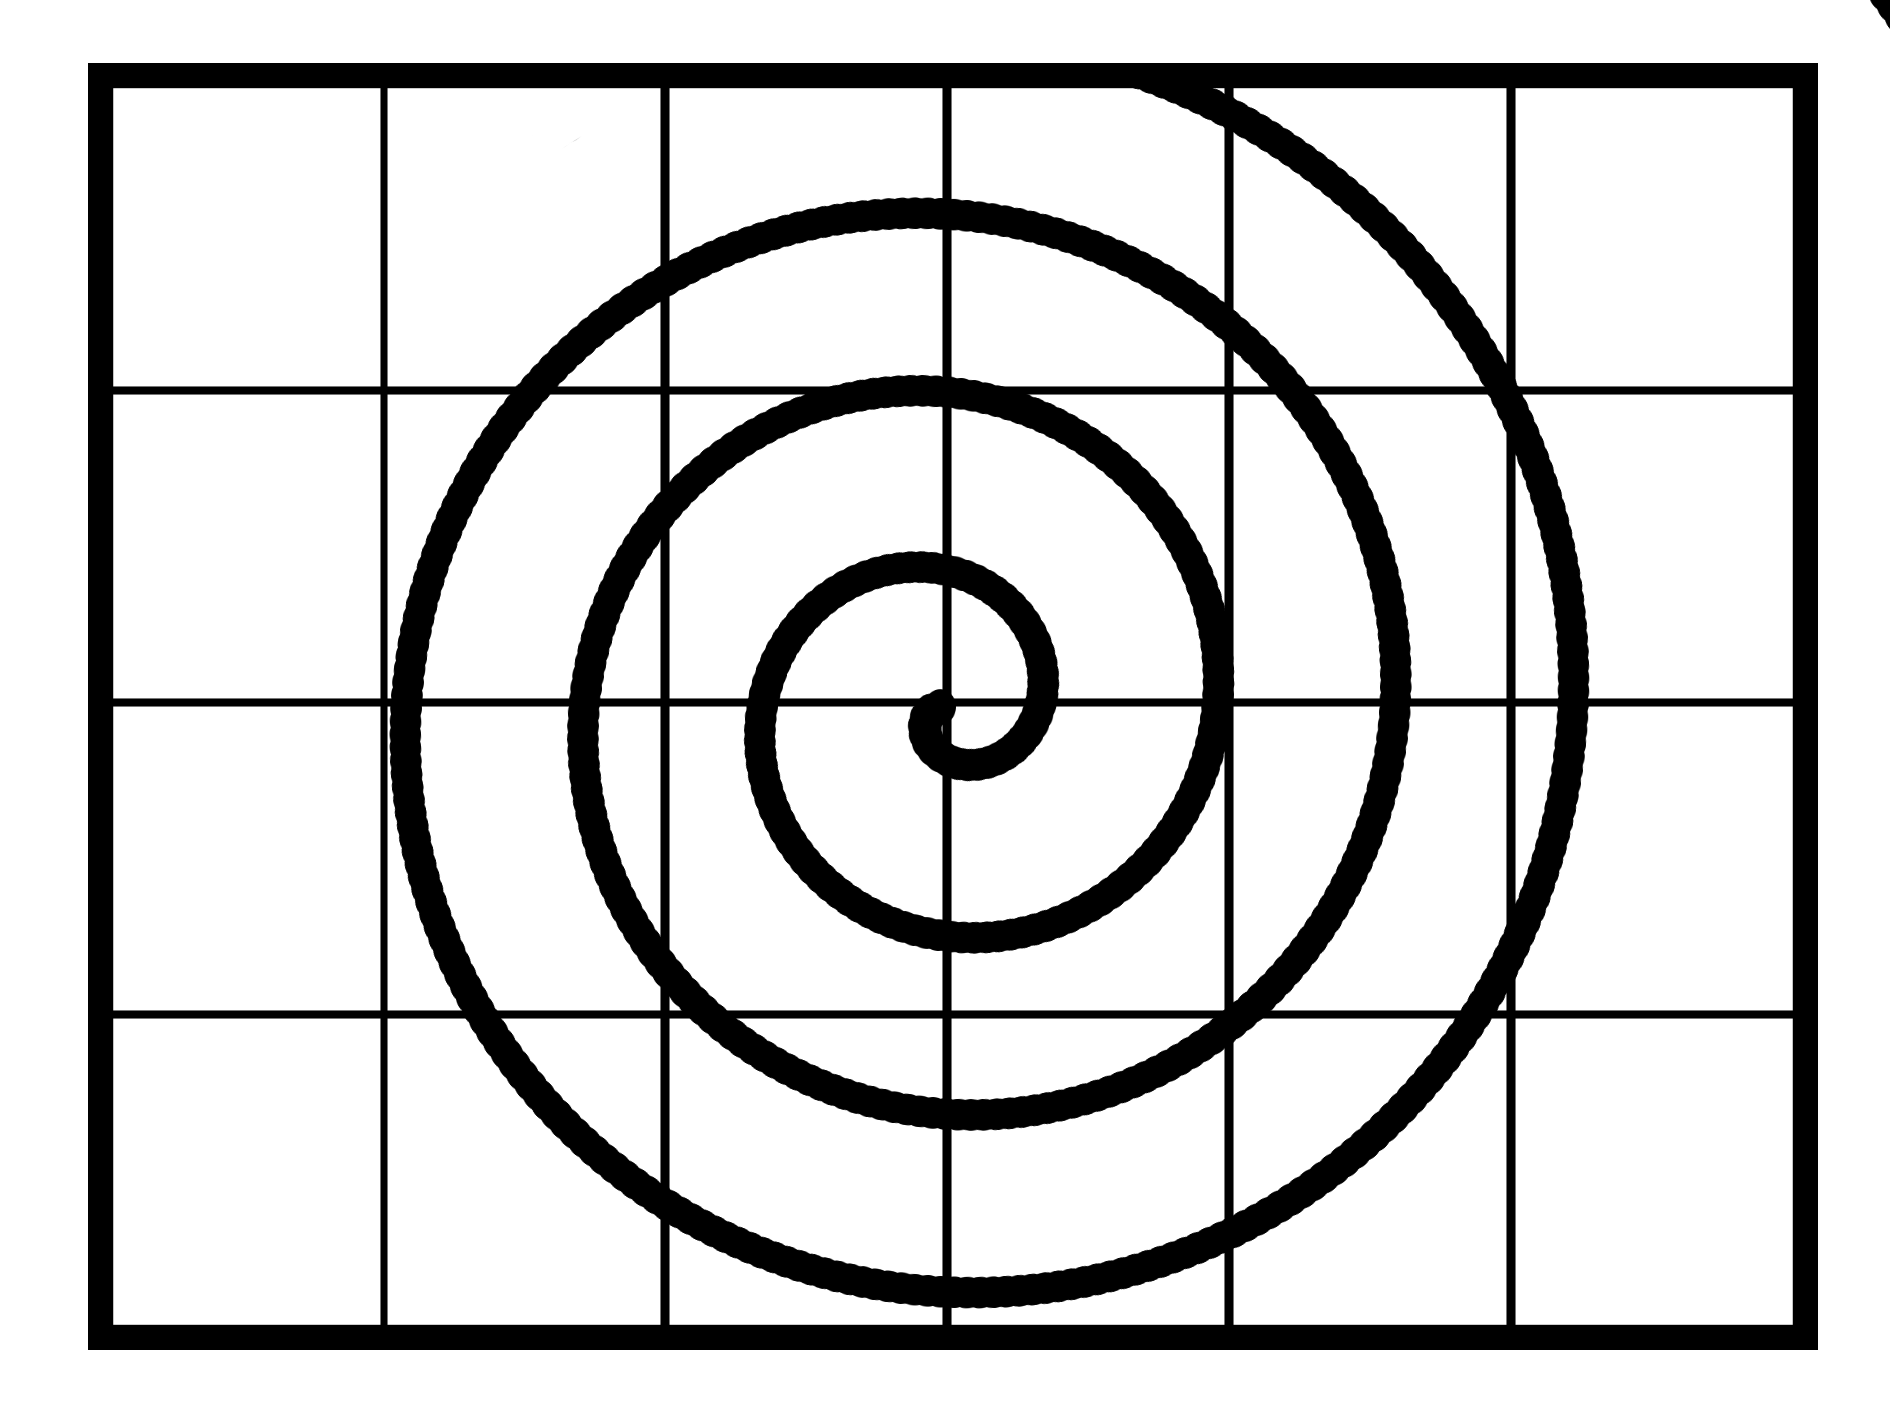
\includegraphics[width=5cm]{img/spiral.png}
	\centering
	\caption{Spiral walk}
	\label{fig:3}
\end{figure}
\subsubsection{Random walk}
The random walk is a very simple algorithm that only needs a simple front bumper sensor.  The robot cleaner just moves in any direction until it hits an obstacle and the front bumper is pressed. When the bumper is pressed the robot cleaner generates a pseudo-random number which decides how much the robot cleaner should turn. From here the algorithm starts over.
(Algorithm.~\ref{alg:rwalk}) is a direct translation from the random walk flowchart from hasan's report \parencite{hasan}.
\\\\
\begin{algorithm}[H]
	\SetAlgoLined
	Move forward
	
	Let one roboUnit = the diameter of the robot
	
	\eIf{collision detected}{
		
		Move backwards one roboUnit
		
		Turn 180 degrees + or - random(90 degrees) 
	}

	\caption{Random Walk}
	\label{alg:rwalk}
	
\end{algorithm}
\bigskip
\noindent  (Figure.~\ref{fig:rwalk}) depicts how one of the paths the generated by the algoritm might look like. 
\begin{figure}[H]
	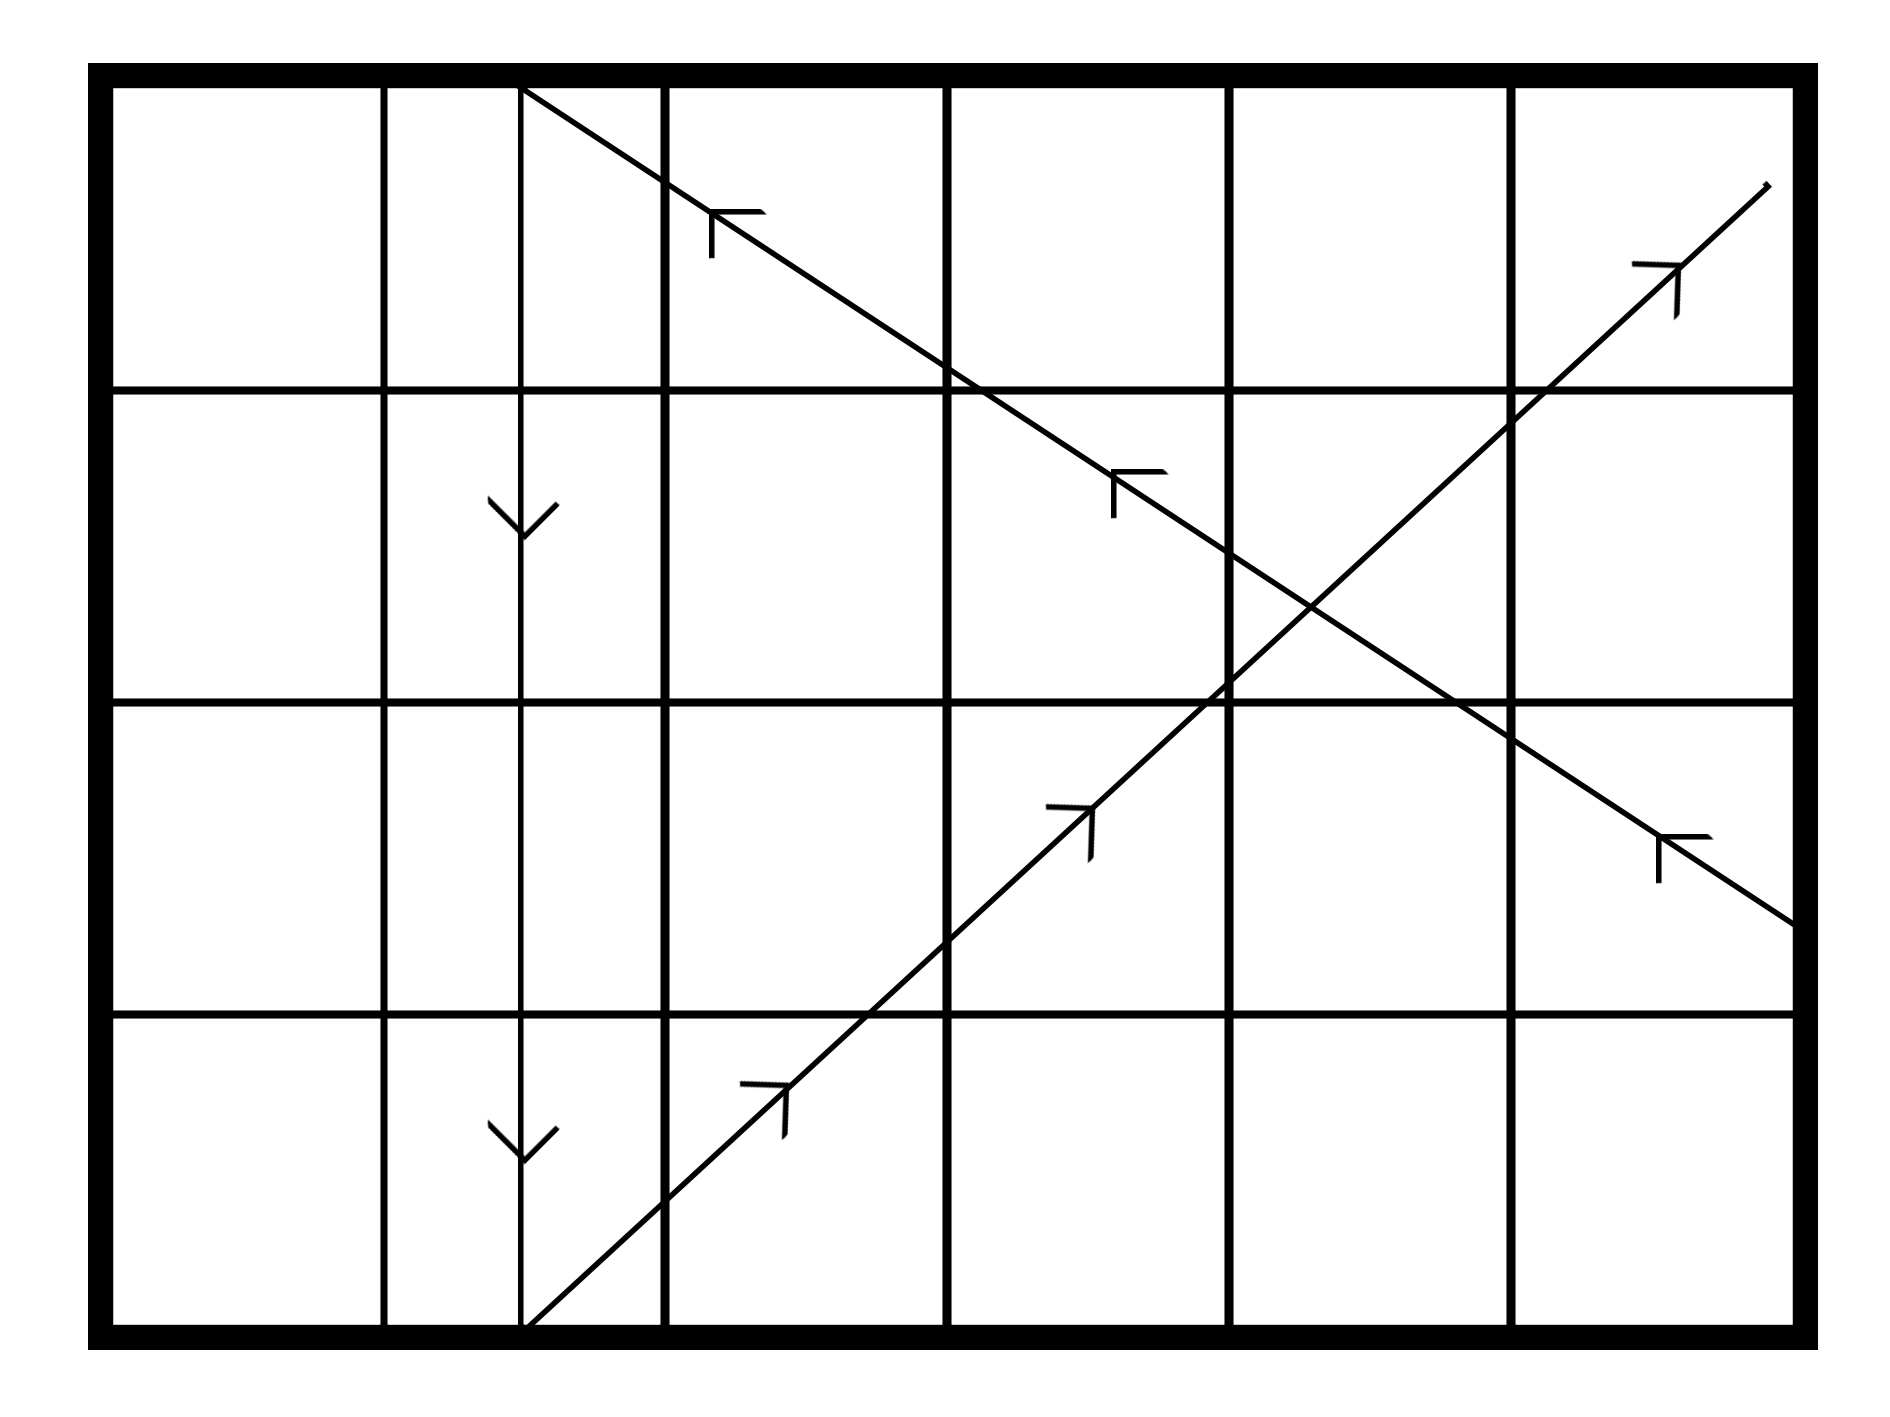
\includegraphics[width=5cm]{img/rwalk.png}
	\centering
	\caption{Random walk}
	\label{fig:rwalk}
\end{figure}
\subsubsection{Wall follow}
The wall follow algorithm moves forward until the front bumper is
triggered, at which point it turns 180 degrees away from the wall and then starts a circular motion until it hit the walls again.The algorithm repeats this procedure until the entire room has been covered along the Walls. This algorithm stays near the walls and never sways far away from them, this means it only cleans the perimeter of the room \parencite{hasan}. 
This algorithm is seldom used alone but instead combined with the spiral algorithm. 
(Algorithm.~\ref{alg:wfoll}) is a interpretation of the wall follow flowchart from hasan's report \parencite{hasan} and the half circle motion is from my own robot cleaner \parencite{centurion}.
\\\\
\begin{algorithm}[H]
	\SetAlgoLined
	Move forward
	
	\eIf{collision detected}{
		
		Turn 180 degrees
		
		Move forward with a pre set angle speed
	}
	
	\caption{Wall follow}
	\label{alg:wfoll}
	
\end{algorithm}
\bigskip
\noindent (Figure.~\ref{fig:wfoll}) depicts how one of the paths generated by the algoritm might look like.
\begin{figure}[H]
	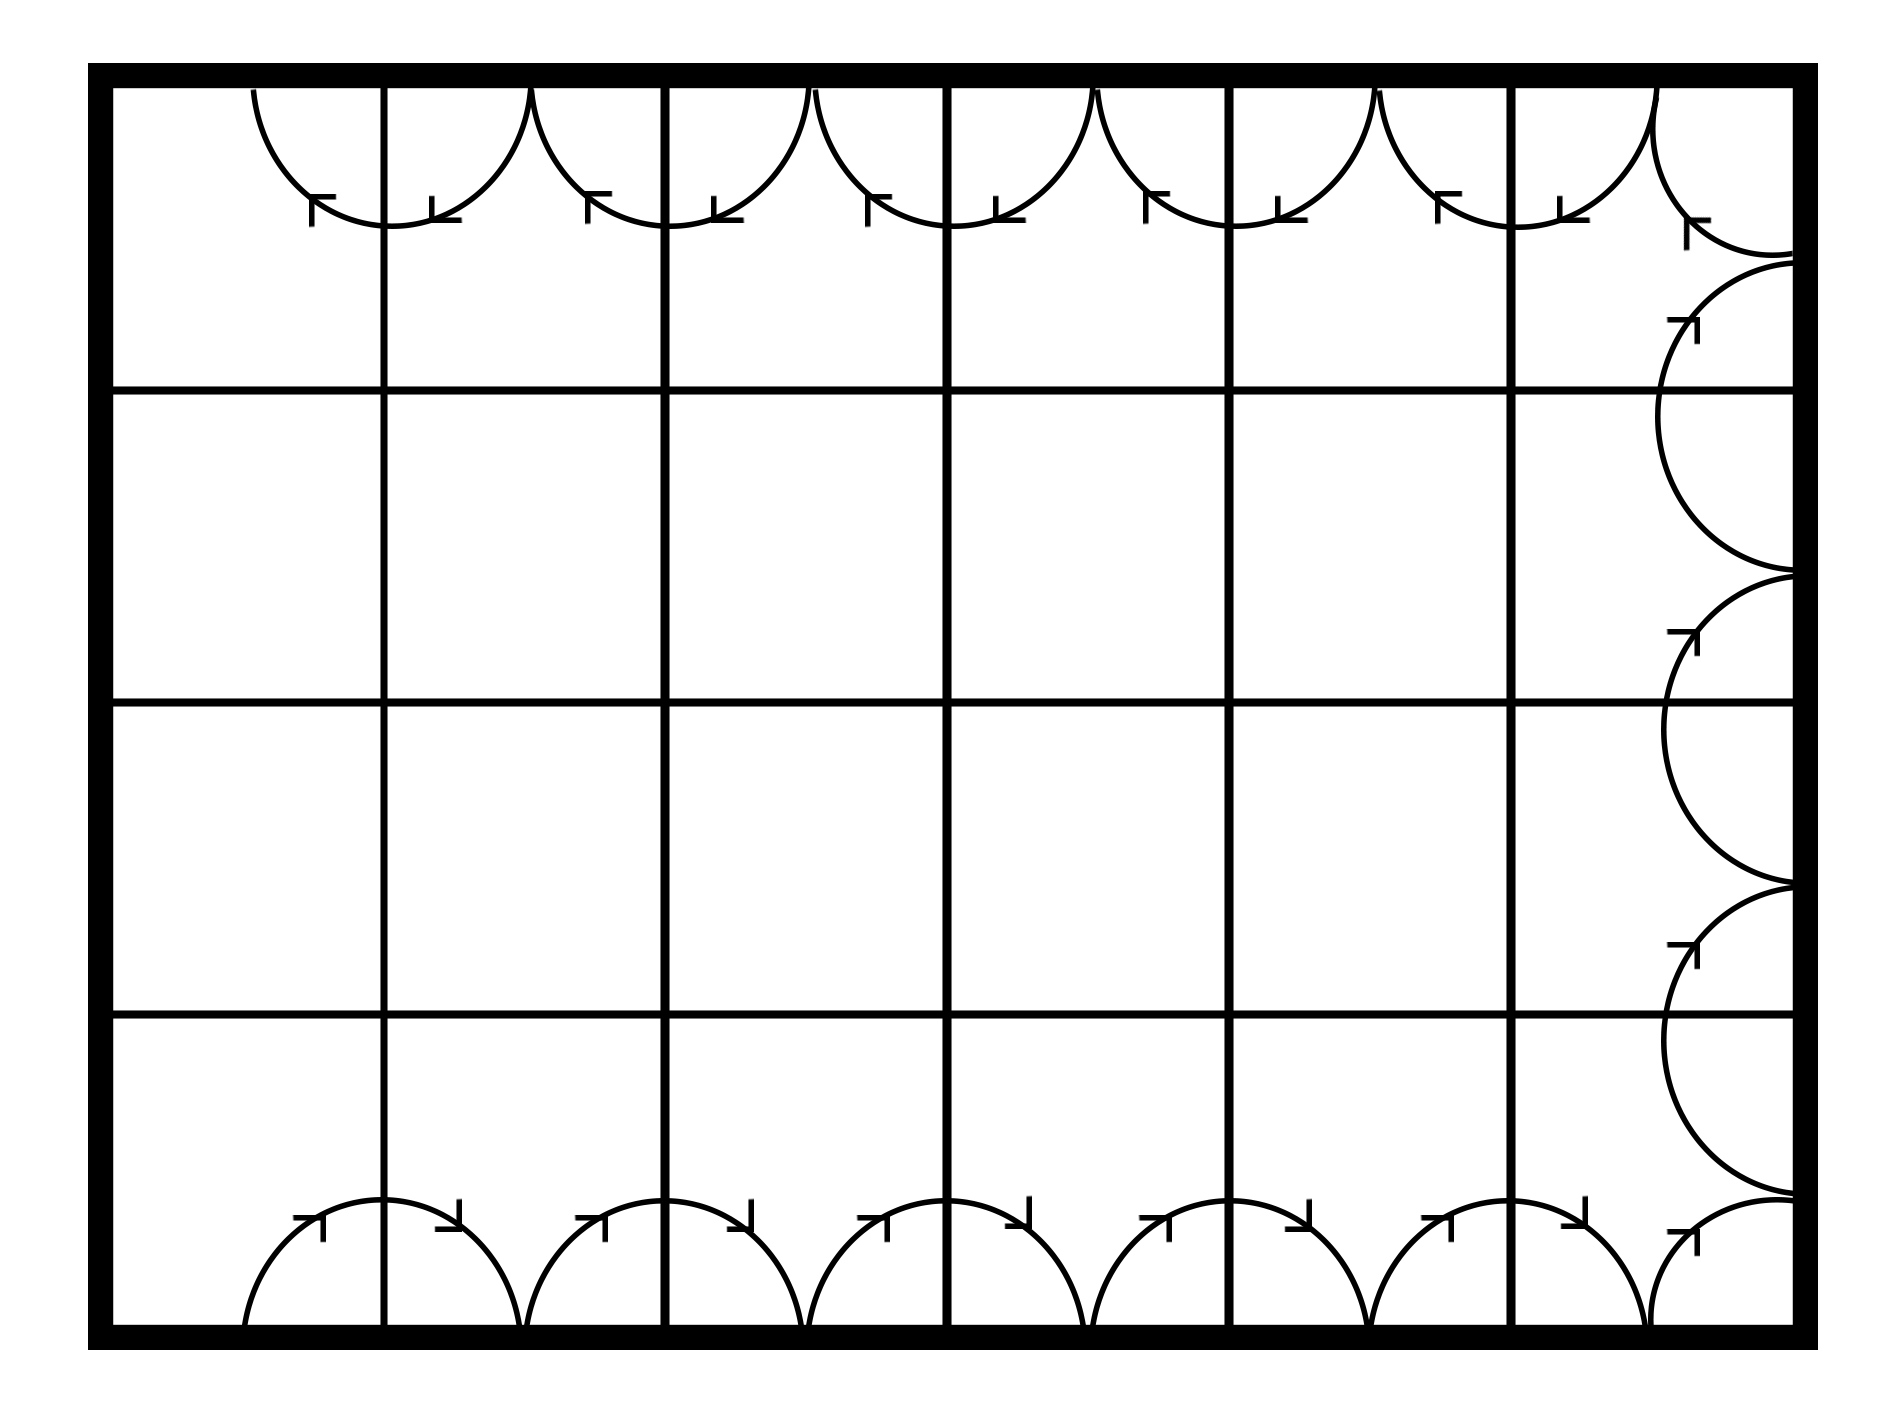
\includegraphics[width=5cm]{img/wfoll.png}
	\centering
	\caption{Wall follow}
	\label{fig:wfoll}
\end{figure}
\subsubsection{Spiral + Wall follow}
This is a combination of the spiral and the wallfollow algorithm. When the front bumper is triggered while using the spiral algorithm, the robot cleaner switches to the wall follow algorithm. This is useful for when the robot cleaner is starting in the middle using spiral. The algorithm switches only once. So when going from spiral to wall follow there is no way to switch back to spiral.

\subsubsection{All combined}
The all combined algorithm is using all of the above described algorithms and using a timer to change between them. Starting with boustrophedon, switching over to random walk and from there switching to spiral and when the front bumper is triggered switching to wall follow and then starting the whole cycle over again.

\section{Problem statement}

Robots with only one bumper sensor have limited options in what algorithms can be used to get 
coverage in a room. \emph{This work aims to perform a series of empirical tests to classify which of these 
algorithms get most coverage or if a specific combination of these algorithms is better than another 
combination.}
My hypothesis is that Boustrophedon will perform better in every room that only has 90 degrees 
corners and with a maximum of 2 pieces of furniture. If that is the case and you have a sparse funitured room 
no algorithm except boustrophedon is needed to get a coverage of 80\% as fast or faster than all the algorithms combined.
\\\\
The robot cleaner in this simulation only has a front bumper which allows it to sense when it hits 
an obstacle, no other sensors are present. This means the robot cleaner has no knowledge of the 
world at the beginning and no knowledge at the end.
Boustrophedon, spiral and wall follow are all deterministic algorithms while random walk is not.
Floor space will be represented by white pixels and walls and obstacles will be black pixels and 
already cleaned area will be painted with red pixels.

\chapter{Method}
\section{Simulation}
By making a simulation of a robot cleaner with only a bumper sensor and  providing it with a room, the simulation is able to compare and present which algorithm is best suited for that type of room. Other ways to test this by using a real robot cleaner, and clean real rooms. As far as we know there are no funding for this, and making a simulation makes it possible to try out each algorithm separatly and also come up with new algorithms.

The simulation is written in Python and is a graphical implementation of the robot and the room, the
robot only has one sensor which is a front bumper that spans 120 degrees on the front of the robot \parencite{hasan}.

The robot cleaner leaves a trail of red to show where the robot cleaner has cleaned (Figure.~\ref{fig:midrun}).
Due to how computational heavy counting colored pixels, every second the algorithm runs the simulation counts how much coverage the robot has accumulated. 

At 100 seconds running time, the simulation ends and the results are presented to the user. 
\\\\
The algorithms used in this simulation are constructed using the flow charts found in Path Planning Algorithm Development for Autonomous Vacuum Cleaner Robots \parencite{hasan}.

\begin{figure}[H]
	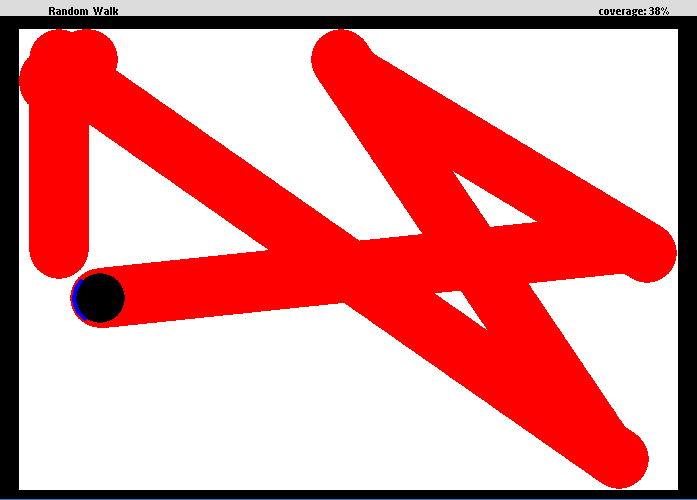
\includegraphics[width=7cm]{img/midrun.png}
	\centering
	\caption{The simulator in running the random walk algorithm}
	\label{fig:midrun}
\end{figure}

\subsection{Rooms}
There are four different types of rooms, two of which are entirely empty and two that are sparsely furnitured. Corners are only angled at 90 degrees.
The rooms are in the form of a bitmap image file which makes it easy to create new rooms for the 
simulator to run.
\\\\
This is the standard room, rectangular and empty.
\begin{figure}[H]
	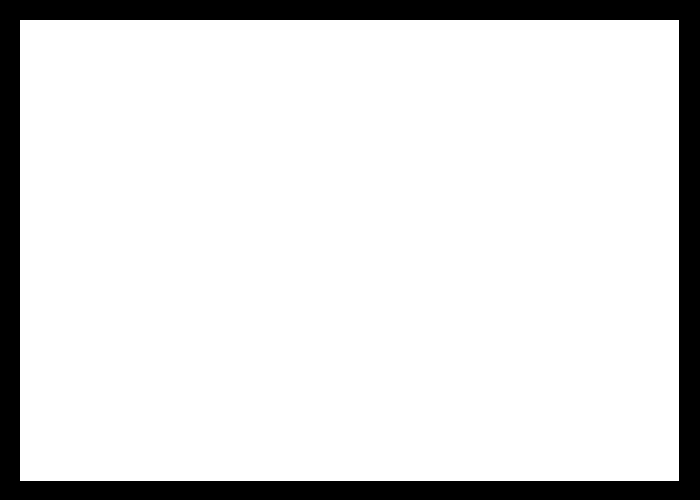
\includegraphics[width=7cm]{img/room.png}
	\centering
	\caption{Room 1}
\end{figure}
This ''room'' consists of several spaces with half walls and small corners that divide the room.
\begin{figure}[H]
	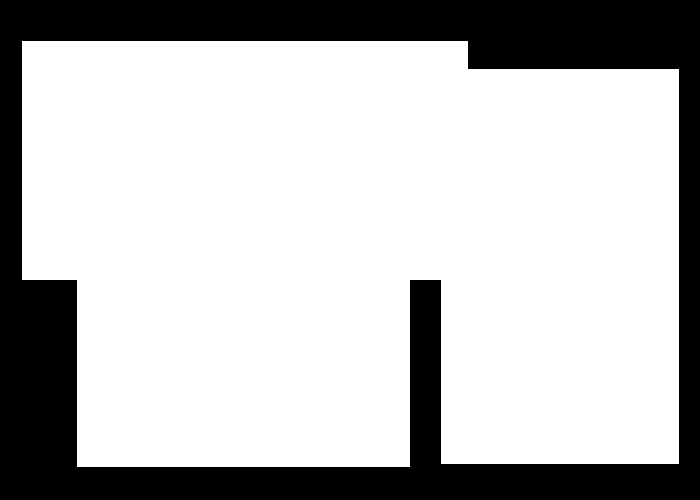
\includegraphics[width=7cm]{img/room2.png}
	\centering
	\caption{Room 2}
\end{figure}
This is the standard room but furnished with a small sofa and an arm chair.
The sofa and the arm chair are represented by four points in the room since that is where the legs are. The sofa and the arm chair are tall enough for the robot cleaner move underneath them. 
\begin{figure}[H]
	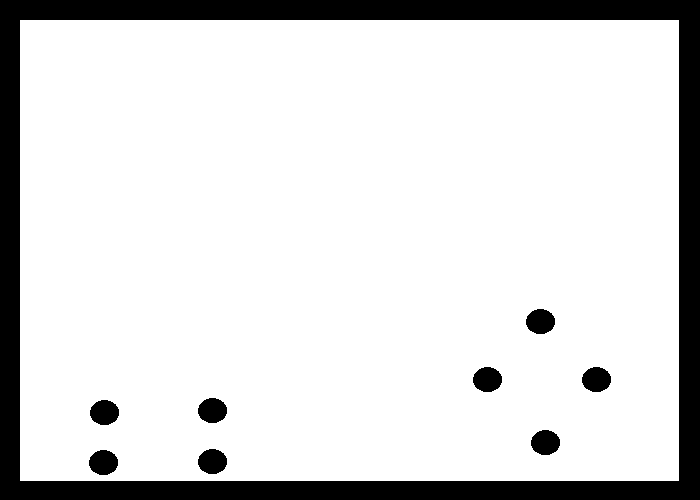
\includegraphics[width=7cm]{img/roomfurn.png}
	\centering
	\caption{Room 3}
\end{figure}
This narrow passages with a sofa and an arm chair.
\begin{figure}[H]
	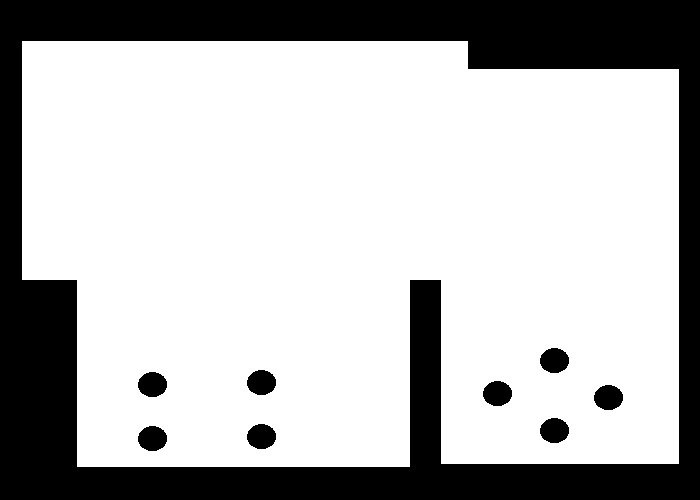
\includegraphics[width=7cm]{img/room2furn.png}
	\centering
	\caption{Room 4}
\end{figure}
\bigskip 
\noindent The simulation starts by counting the area of the room by counting the white pixels inside of the walls, then the algorithm to use is chosen. 



\section{Benchmarks}
As a benchmark, the simulator will run all four of the algorithms with a timer to switch between them. This is what some cheap robot cleaners use \parencite{hasan}.
This is used to as a control to compare if any of the other algorithms are good enough to be used alone.


\chapter{Results}
The results come from running the simulation several times for each type of room. The non-deterministic algorithms were tested by computing the
mean of 10 separate runs, while the deterministic algorithms were 
tested with a single run.
The non-deterministic algorithms are Random Walk and All Combined, all other algorithms will get the same result every time.
The reason some algorithms get stuck at a certain percentage of coverage is that the robot cleaner got stuck and this is how the algorithms should work acording to the flowchart \parencite{hasan}.
\section{Room type 1}
These are the result from room type 1, the empty room. Starting in a corner (Figure.~\ref{fig:corner1}), and starting in the middle of the room (Figure.~\ref{fig:middle1}).
\begin{figure}[H]
	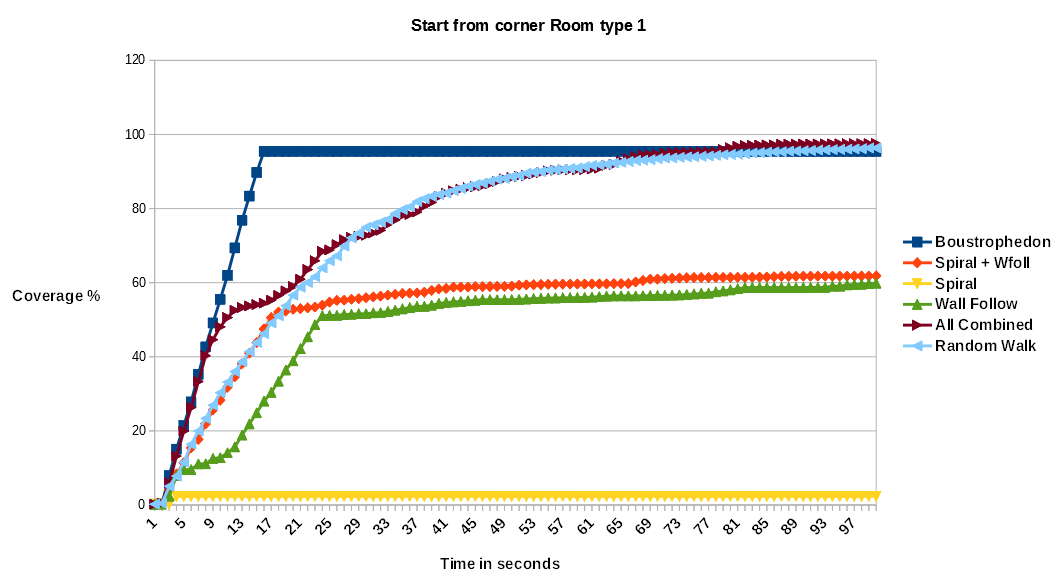
\includegraphics[width=15cm]{img/cornerroom1chart.png}
	\centering
	\caption{Results when starting in a corner in room 1}
	\label{fig:corner1}
\end{figure}
\begin{figure}[H]
	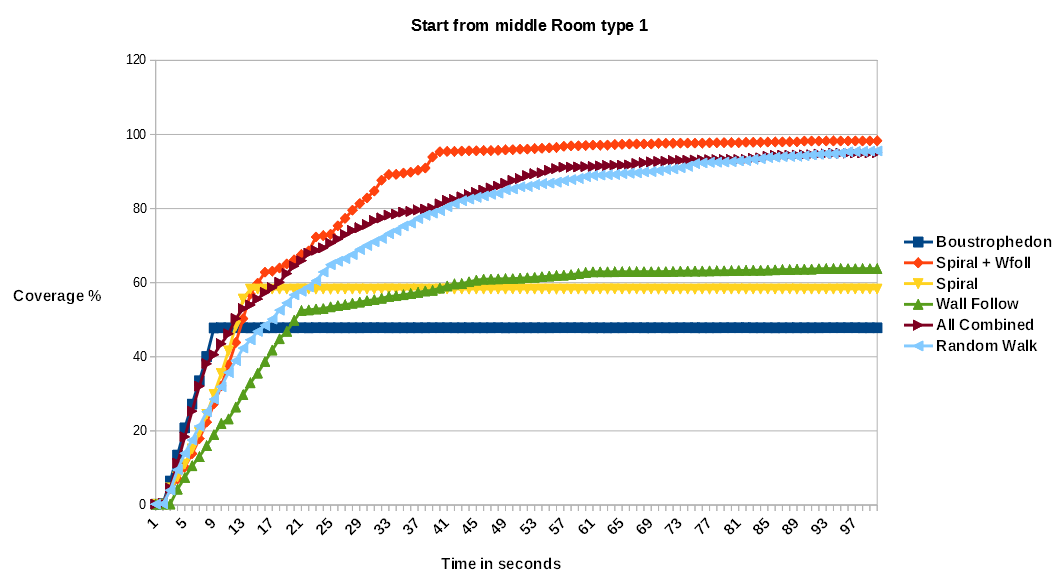
\includegraphics[width=15cm]{img/middleroom1chart.png}
	\centering
	\caption{Results when starting in the middle in room 1}
	\label{fig:middle1}
\end{figure}
\section{Room type 2}
These are the result from room type 2, the room with half walls and small corners. Starting in a corner (Figure.~\ref{fig:corner2}), and starting in the middle of the room (Figure.~\ref{fig:middle2}).
\begin{figure}[H]
	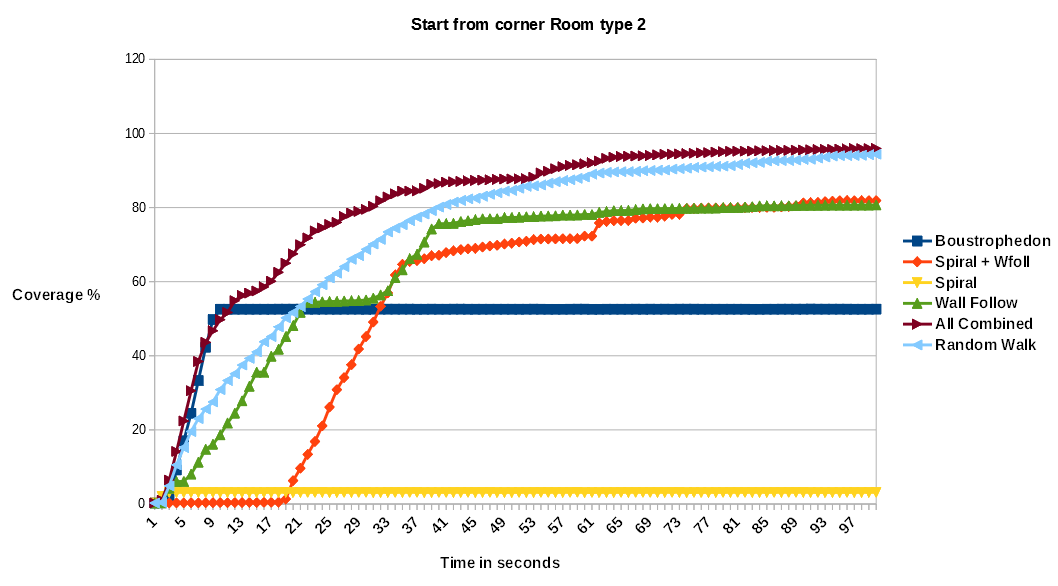
\includegraphics[width=15cm]{img/cornerroom2chart.png}
	\centering
	\caption{Results when starting in a corner in room 2}
	\label{fig:corner2}
\end{figure}
\begin{figure}[H]
	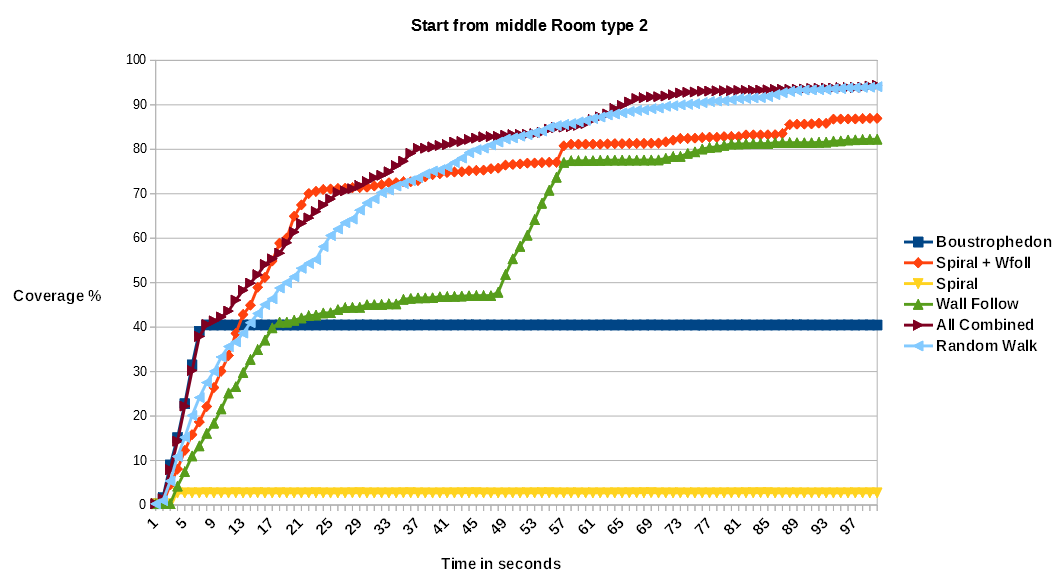
\includegraphics[width=15cm]{img/middleroom2chart.png}
	\centering
	\caption{Results when starting in the middle in room 2}
	\label{fig:middle2}
\end{figure}
\section{Room type 3}
These are the result from room type 3, the standard room but furnished. Starting in a corner (Figure.~\ref{fig:corner3}), and starting in the middle of the room (Figure.~\ref{fig:middle3}).
\begin{figure}[H]
	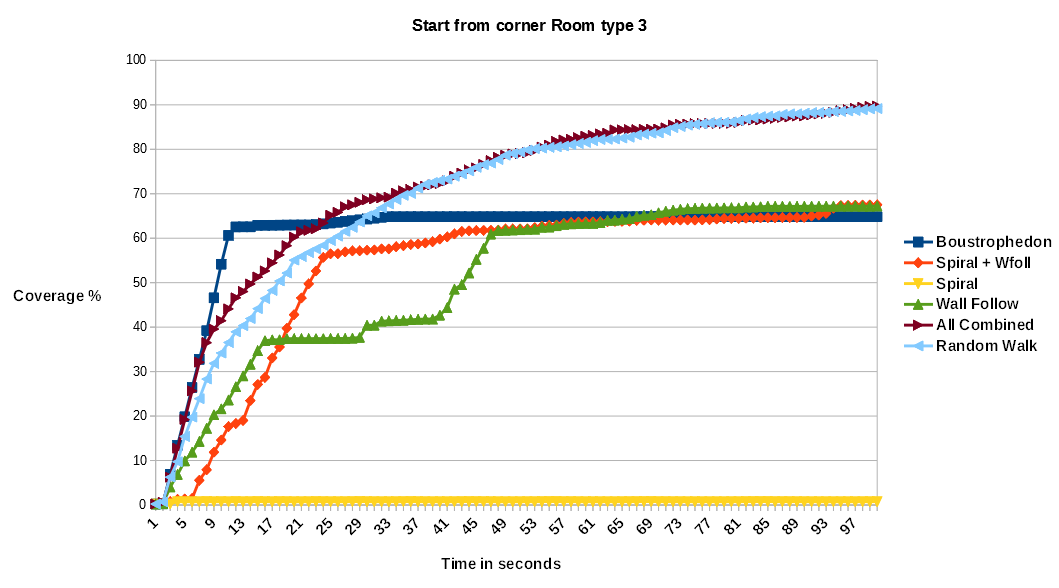
\includegraphics[width=15cm]{img/cornerroom1furnchart.png}
	\centering
	\caption{Results when starting in a corner in room 3}
	\label{fig:corner3}
\end{figure}
\begin{figure}[H]
	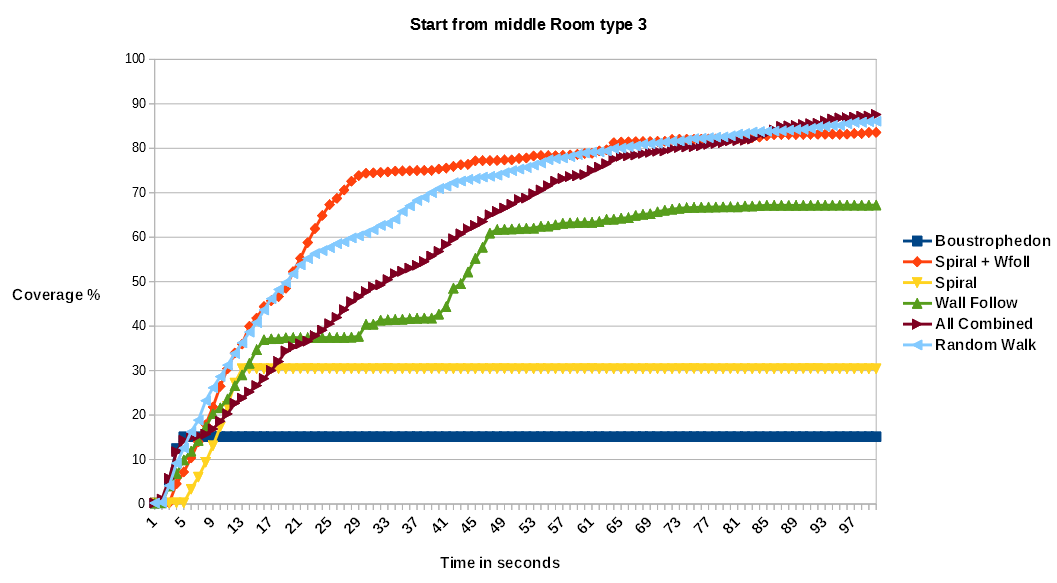
\includegraphics[width=15cm]{img/middleroom1furnchart.png}
	\centering
	\caption{Results when starting in the middle in room 3}
	\label{fig:middle3}
\end{figure}
\section{Room type 4}
These are the result from room type 4, the room with half walls and small corners when furnished. Starting in a corner (Figure.~\ref{fig:corner4}), and starting in the middle of the room (Figure.~\ref{fig:middle4}).
\begin{figure}[H]
	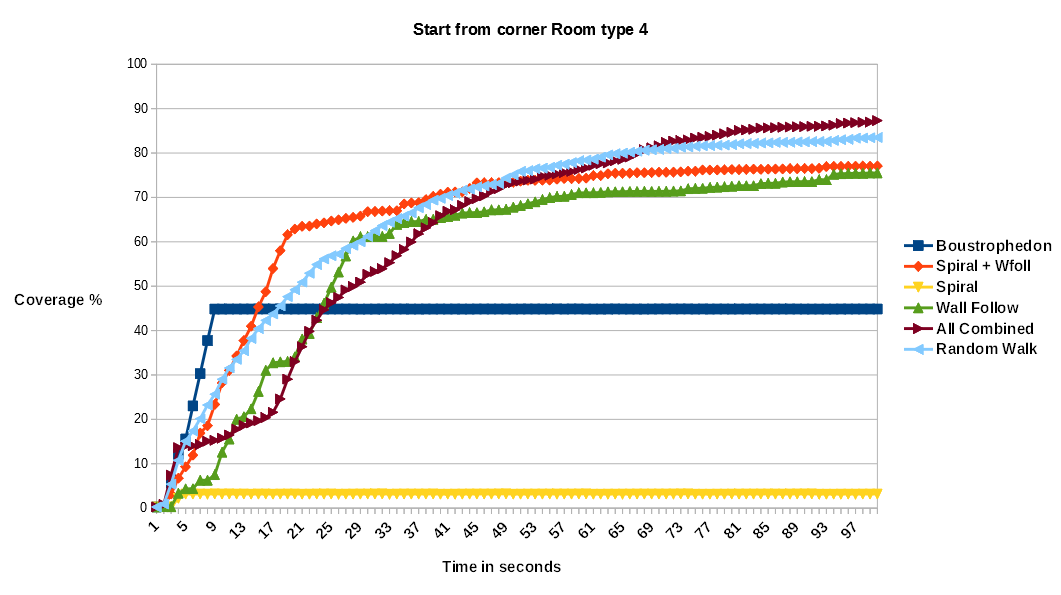
\includegraphics[width=15cm]{img/cornerroom2furnchart.png}
	\centering
	\caption{Results when starting in a corner in room 4}
	\label{fig:corner4}
\end{figure}
\begin{figure}[H]
	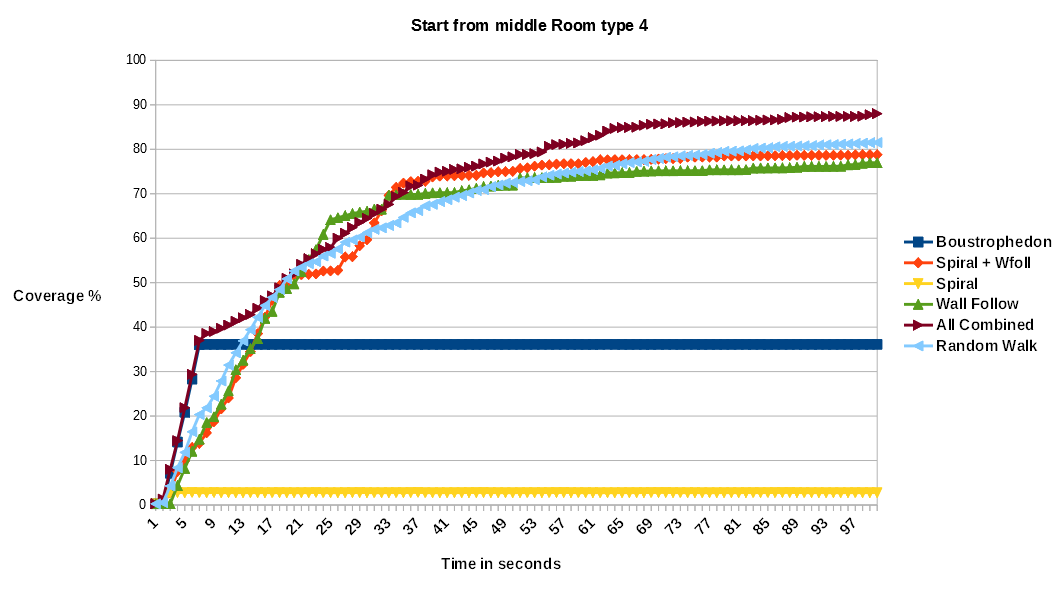
\includegraphics[width=15cm]{img/middleroom2furnchart.png}
	\centering
	\caption{Results when starting in the middle in room 4}
	\label{fig:middle4}
\end{figure}
\chapter{Discussion}
Most of the time, the non-deterministic algorithms got stuck and could not move past the obstacle in their way. Especially spiral which is terrible if the robot cleaner does not start near the middle of the room. Even boustrophedon got stuck a lot of time, and when the robot cleaner hit the most right wall the boustrophedon could not do anything.
The implementation I found of the boustrophedon algorithm did not really meet my expectations, maybe that is just because I did not have enough information about the boustrophedon. However random walk surprised a whole lot. I originally thought that random walk would travel where it has already been befor and therefore clean already clean space, and it does. However it is not that ineffective.
\\\\
\blue{discuss improvements to boustrophedon. }
\chapter{Conclusion}
Boustrophedon by itself is no enough to clean rooms, unless the room is totally empty and the robot cleaner starts in the southern most left corner of the room.
\\\\
\blue{write about the idea of improved boustrophedon}
\printbibliography[heading=bibintoc] % Print the bibliography (and make it appear in the table of contents)

\appendix

\chapter{Unnecessary Appended Material}

\end{document}
